% !TEX root = flows.tex

\section{Introduction}\label{S:intro}

de Rham cohomology has long been lauded as a perfect cohomology theory by champions such as Sullivan \cite{sullivan1977infinitesimal} and Bott \cite{BoTu82}.
A combination of geometric underpinning and commutativity at the cochain level make it a remarkably effective tool for many applications of rational homotopy theory.
Over the integers, submanifolds and intersection (and their generalizations) in various settings provide geometrically meaningful cochains \cite{Lipy14} with a partially defined commutative product \cite{Joyc15, medina2022foundations}.
But the obstructions to commutativity witnessed by Steenrod operations show that intersection alone cannot capture the cochain quasi-isomorphism type multiplicatively without additional machinery, such as a combination of McClure’s partial intersection algebras \cite{McCl06} and Wilson’s algebraic rectification \cite{Wils10}. One of our goals is to provide a more direct geometric reconciliation of these structures.

In this paper we start to marry two imperfect theories, relating multiplicative structures of, on one hand, geometric cochains defined using manifolds with corners, and, on the other, standard cubical cochains.
The comparison chain map $\cI$ between these ``analog" and ``digital" presentations of ordinary cohomology of a closed manifold is defined through counting intersections of geometric cochains with a given cubulation. With the proper definitions, which we set up in detail in \cref{S:geometric cochains}, the map $\cI$ is a quasi-isomorphism.
In the domain of this comparison map there is a natural partially defined product given by transverse intersection, whereas in the target the product structure is induced from the Serre diagonal, a cubical analogue of the Alexander--Whitney diagonal in the simplicial setting.
Both of these multiplicative structures induce the standard cup product in cohomology, but at the cochain level they are not immediately compatible.
We bind them using the flow of a vector field canonically defined using the cubulation.

\begin{figure}[h]
	\centering
	\hfill
	\begin{subfigure}[b]{0.45\textwidth}
		\hspace*{-9pt}
		\includegraphics[scale=.6]{figures/logistic.pdf}
		\caption{The logistic vector field on $\interval^2$.
		Because logistic vector fields are consistent across cubical faces, this vector field extends to any cubulated surface.}
	\end{subfigure}
	\hspace{0.2 in}
	\begin{subfigure}[b]{0.45\textwidth}
		\raisebox{9.5pt}{\documentclass[tikz,border=2mm]{standalone}
\usepackage{tikz}

\definecolor{red}{rgb}{1,.5,.6}
\definecolor{blue}{rgb}{.5,.5,1}

\begin{document}
	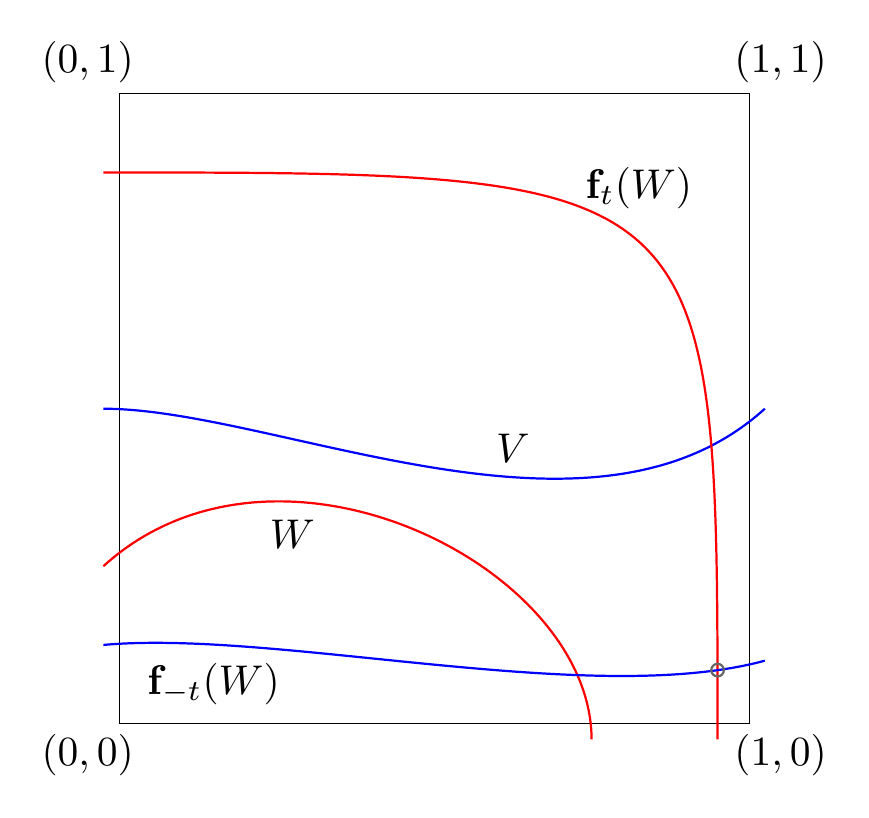
\begin{tikzpicture}[scale = 2]

	\draw (0,0) -- (0,4) -- (4,4) -- (4,0) -- (0,0);

	\draw[red, thick] (-.1,1) .. controls (1,2) and (3,1).. (3,-.1);
	\draw[blue, thick] (-.1,2) .. controls (1,2) and (3,1).. (4.1,2);
	\draw[red, thick] (-.1,3.5) .. controls (3.8,3.5) .. (3.8,-.1);
	\draw[blue, thick] (-.1,.5) .. controls (1,.6) and (3,.1).. (4.1,.4);

	\node[scale=1.5] at (-.2, -.2) {$(0,0)$};
	\node[scale=1.5] at (4.2, -.2) {$(1,0)$};
	\node[scale=1.5] at (4.2, 4.2) {$(1,1)$};
	\node[scale=1.5] at (-.2, 4.2) {$(0,1)$};

	\node[scale=1.5] at (1.1, 1.2) {$W$};
	\node[scale=1.5] at (2.5, 1.75) {$V$};
	\node[scale=1.5] at (3.3, 3.4) {$\mathbf f_t(W)$};
	\node[scale=1.5] at (.6, .25) {$\mathbf f_{-t}(W)$};

	\draw[color=black!60, thick](3.8,.34) circle (.04);
	\draw[circle,fill,radius=1000pt,black] (4,2);
	\end{tikzpicture}
\end{document}}
		\caption{The intersection of $W$ and $V$ is not compatible with the corresponding cubical cup product, but that of $\f_t(W)$ and $\f_{-t}(V)$ is.}
	\end{subfigure}
	\caption{The logistic vector field and the impact of its flow on intersections.}
	\label{F:logistic}
\end{figure}

The basic idea of the construction is given in \cref{F:logistic}.
The logistic vector field is pictured in part (A) of the figure with its time $t$ flow denoted by $\f_t$.
Part (B) of the figure illustrates the main idea of how the flow reconciles multiplications.
Here $W$ and $V$ are manifolds with corners mapping to a closed manifold $M$ which we assume cubulated, focusing the picture on a single square.
As explained in \cref{S:geometric cochains}, such maps represent geometric cochains of $M$, and integer coefficients can be considered if additional (co)orientation data is included.
A geometric cochain that is transverse to the cubulation, as we are assuming $W$ and $V$ are, defines a cubical cochain, say $\cI(W)$, by a count of signed intersection numbers where $W$ intersects a cubical face of complementary dimension.
The picture shows that with mod-two coefficients $\cI(W)$ evaluates to 1 on the bottom and left edges, while $\cI(V)$ evaluates to 1 on the left and right edges.
As explained in \cref{S:cubical topology}, because the bottom edge and right edge form an ``initial-terminal'' pair of faces of the square, the Serre diagonal construction gives that $\cI(W) \sms \cI(V)$ evaluates to 1 on the square.
As $W$ and $V$ do not intersect each other, their intersection product evaluates to 0 on the square, and thus disagrees with the cup product at the cochain level.
Yet, for $t$ sufficiently large, $\f_t(W)$ and $\f_{-t}(V)$ intersect while maintaining $\cI(W) = \cI(\f_t(W))$ and $\cI(V) = \cI(\f_{-t}(V))$, now yielding agreement between the intersection and cup products at the cochain level.

Our main result is that logistic flow performs such reconciliation in general.
We write $W \times_MV$ for the fiber product of $W$ and $V$ over $M$, which gives rise to the partially defined product on geometric cochains, defined when $W$ and $V$ are transverse.
With this notation we now present the main result of this work.

\begin{restatable}{theorem}{maintheorem}\label{T:main theorem}
	Let $M$ be a cubulated closed manifold and $W$ and $V$ two compact co-oriented manifolds with corners over $M$ which are transverse to the cubulation. Then, for $t$ sufficiently large:
	\begin{enumerate}
		\item $\f_t(W)$ and $\f_{-t}(V)$ are transverse and
		\begin{equation*}
			\cI\left(\f_t(W) \times_M \f_{-t}(V)\right) = \cI\left(\f_t(W)\right) \sms \cI\left(\f_{-t}(V)\right).
		\end{equation*}
		\item $\f_{-t}(W)$ and $\f_t(V)$ are transverse and
		\begin{equation*}
			\cI\left(\f_{-t}(W) \times_M \f_t(V)\right) = (-1)^{|W||V|} \, \cI\left(\f_t(V)\right) \sms \cI\left(\f_{-t}(W)\right),
		\end{equation*}
		where $|W||V|$ is the product of the codimensions of $W$ and $V$ over $M$.
	\end{enumerate}
\end{restatable}

It is classically known that the intersection and cup products are Poincar\'e dual at the level of homology and cohomology, but, to our knowledge, this result is the first to give an explicit connection between these products at the cochain level.

Turning to applications, manifold cochains have primarily been developed as a parallel to, or for application in, string topology \cite{chas1999string}, Floer theory \cite{Lipy08}, and other types of moduli questions \cite{BoJo17}.
More work needs to be done for our viewpoint to connect with these fields, but as they stand, the results of this paper are applicable, for example, in using the bar construction on cochains to define knot invariants through induced maps on configuration spaces \cite{BCSS05, SiWa13, BCKS17}.

Since the logistic flow interpolates between commutative and noncommutative worlds, in future work we plan to connect it to cup-$i$ products \cite{steenrod1947products, medina2022axiomatic, medina2023fast_sq} and higher derived structures \cite{medina2020cartan, medina2021adem, medina2023oddcartan}.
More generally, as has been done for combinatorial cochains \cite{mcclure2003multivariable, berger2004combinatorial, medina2020prop1, medina2022cube_einfty}, our work invites the possibility of defining \mbox{$E_\infty$-structures} on geometric cochains and the description of cohomology operations at the cochain level \cite{medina2021may_st} using geometric language.
We are particularly interested in building on the work of Mandell \cite{mandell2001padic, mandell2006homotopy_type} and others to model homotopy types of manifolds via geometric cochains.

The question of relating vector field flows to finer cochain structures has also recently arisen in mathematical physics \cite{Thor18, Tata20}, but the vector fields in \cite{Tata20} are non-continuous.
Our flow is globally smooth and thus should serve as a strong bridge between physical models, geometry, and topology.

There are two variants of \cref{T:main theorem} which are likely of interest but which will not be addressed in this paper.
First, one can use simplices instead of cubes.
Working with cubulations simplifies our treatment since the logistic flow on standard cubes is given coordinate-wise by the logistic flow on the interval.
But the simplicial version of \cref{T:main theorem} can be proven for simplicial cochains with the Alexander--Whitney product, using the results of this paper and the model of standard simplices as subsets of cubes with non-increasing coordinates.
We leave the details to the interested reader.
Secondly, we conjecture that there is a version of \cref{T:main theorem} in which some finite subcomplex of geometric cochains maps to a version of transverse smooth singular cochains.
Precise formulation of such a comparison map is one of the topics we hope to address in the future, but for now we leave this idea undeveloped.

We begin the paper by reviewing in \cref{S:cubical topology} basic material on cubical structures.
We then describe geometric cochains defined using manifolds with corners, a notion that arises naturally when considering fiber products of manifolds with boundary.
However, for manifolds with corners the boundary of a boundary is not empty, so one must impose a quotient at the cochain level to obtain a cochain complex.
In \cref{S:geometric cochains}, we review the needed parts of this theory as presented in \cite{medina2022foundations} and based on the original definition of Lipyanskiy \cite{Lipy14}.
In \cref{S:logistic}, we then develop logistic vector fields, for which the analysis is thankfully simple to manage.
These vector fields in a sense give a smooth extension of the cubical poset structure, the key combinatorial structure used in defining the cubical cup product.
We put everything together in \cref{S:flow comparison theorem} to prove our main comparison theorem, stated above, which intuitively says that after sufficient time flow intersection yields a ring homomorphism from geometric cochains to cubical cochains.

\section*{Acknowledgments}

The authors thank Mike Miller, for pointing us to \cite{Lipy14}; Dominic Joyce, for answering questions about his work; and the reviewer for a careful and insightful analysis of our paper.